\documentclass[14pt]{extreport}
\usepackage{gost}
%\usepackage{hyperref}
%\usepackage{makecell}
\usepackage{ragged2e}
%\usepackage{graphicx}%Вставка картинок правильная
%\usepackage{float}%"Плавающие" картинки
%\usepackage{wrapfig}%Обтекание фигур (таблиц, картинок и прочего)
%\justifying

\newcolumntype{P}[1]{>{\raggedrightarraybackslash}p{#1}}
\makeatletter
\@addtoreset{figure}{part}% Reset figure numbering at every part
\makeatother
\renewcommand{\thefigure}{\arabic{figure}}% Figure number is part.figure
\renewcommand{\thetable}{\arabic{table}}

%Тут можно вставить дополнительные пакеты

\begin{document}
    \pagestyle{empty} %  выключаем нумерацию
    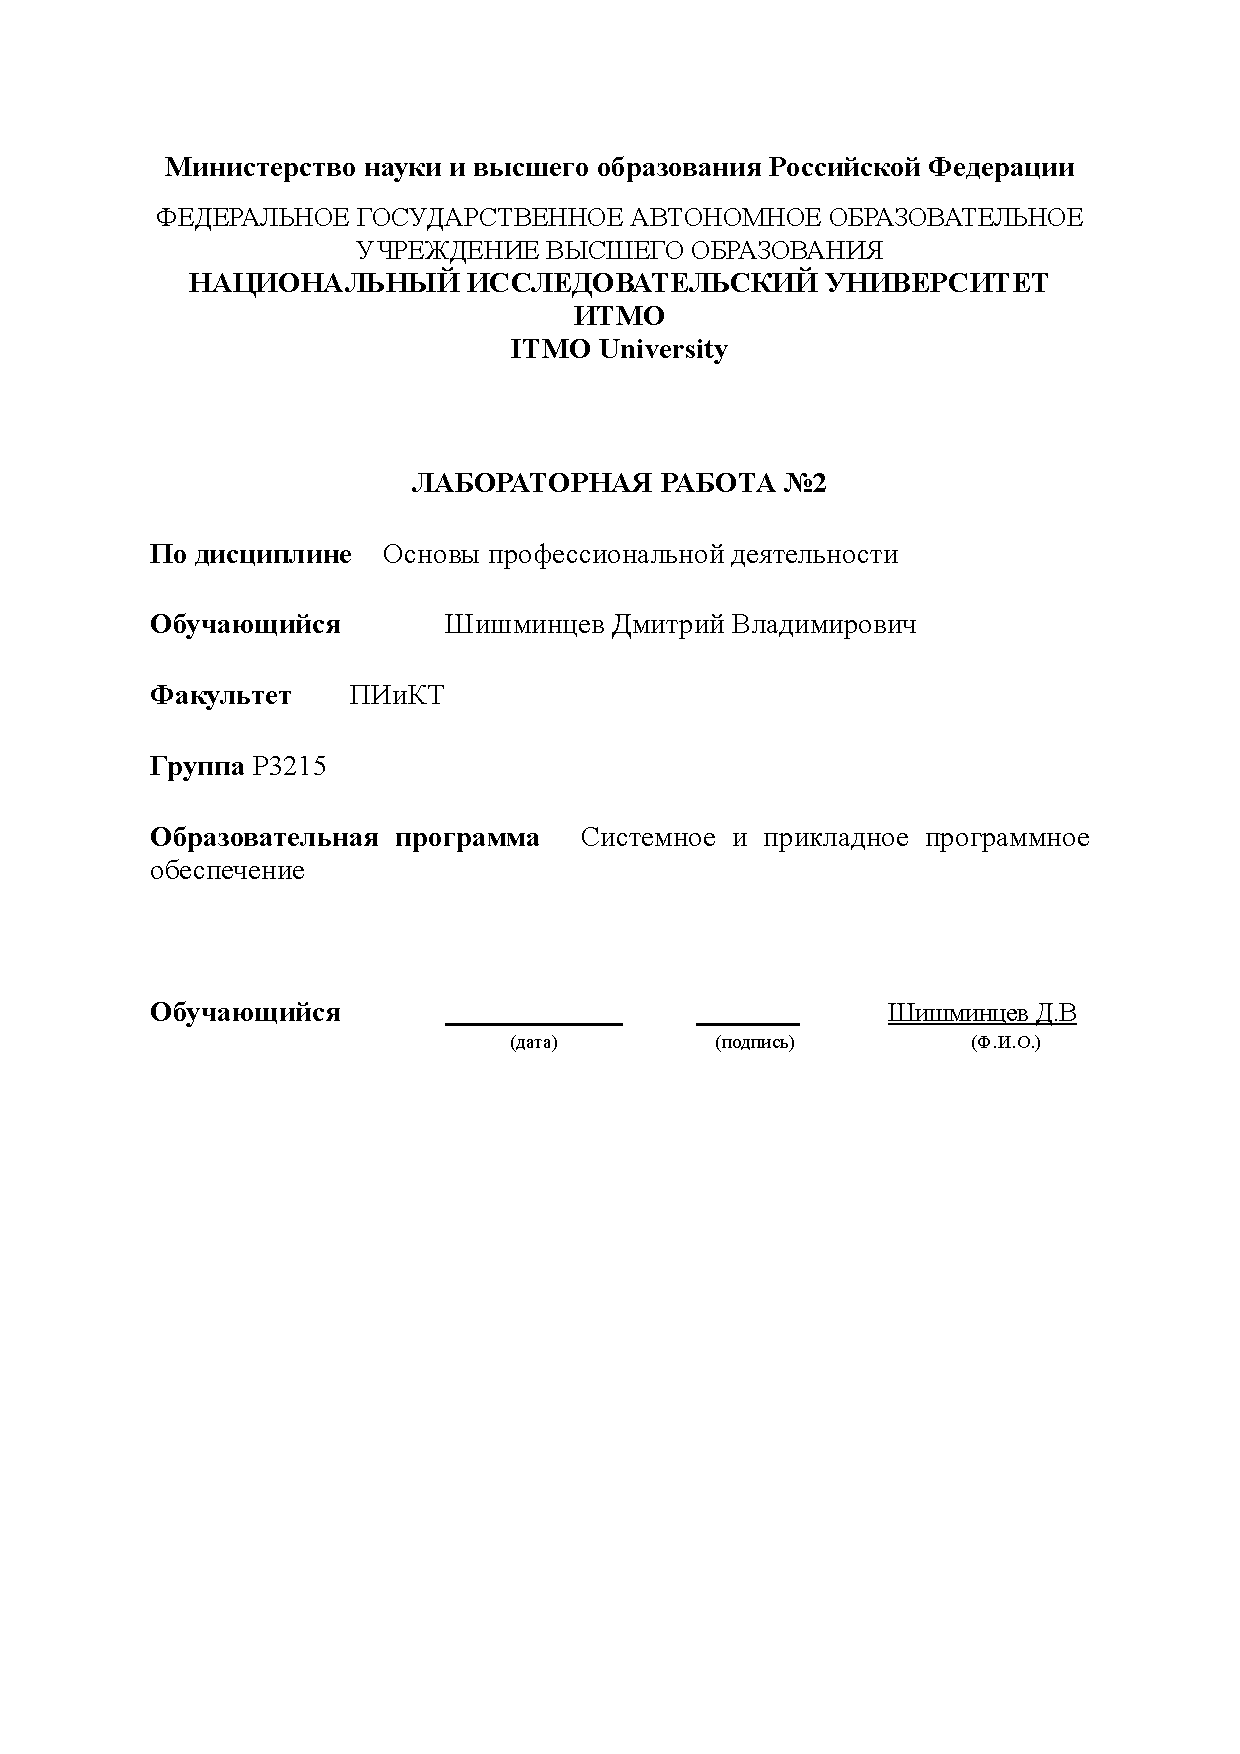
\includepdf[pages=-,pagecommand={}]{title_page.pdf}

    \pagestyle{plain} % включаем нумерацию
    \tableofcontents
    \intro Задание по базовой электронной вычислительной машине (ЭВМ) предполагает анализ программы, определение её функции, области представления и области допустимых значений исходных данных и результатов. В процессе выполнения задания требуется также провести трассировку программы и предложить вариант с уменьшенным числом команд. Этот анализ поможет понять, как программа взаимодействует с данными и как можно оптимизировать её выполнение.

    \chapter{Текст задания}


        \begin{figure}[!h]
            \centering
            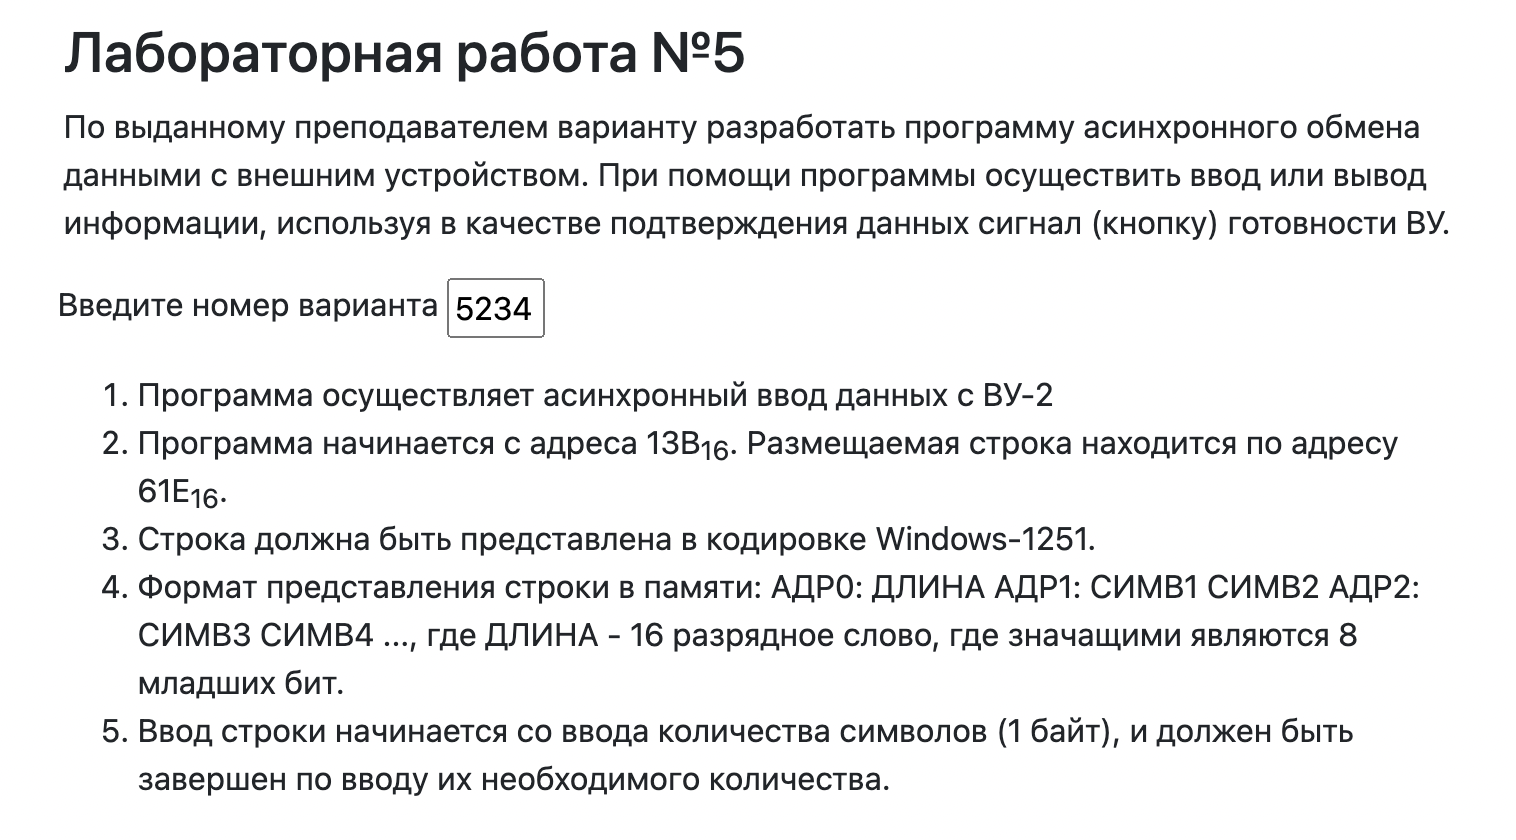
\includegraphics[width=0.8\linewidth]{task.png}
            \caption{Картинка задания}

        \end{figure}


    \chapter{Таблица исходной программы}

            \begin{tabular}{|P{1.5cm}|P{3cm}|P{4cm}|P{5cm}|}
                \hline
                Адрес & Код команды & Мнемоника & Комментарий \\
                \hline
                139& 0000 & TEMP& Временное значение\\
                13A& 0000 & LEN & Длинна \\
                13B& 061E & POINTER & Указатель на начало массива \\ \hline
                13C& 0200 & CLA& 0=>AC \\
                13D& 1205 &LENGTH: IN 5& Чтение из регистров ВУ\\
                13E& 2F40 & AND #0x40& Логической И\\
                13F& F0FD &BEQ LENGTH& Если AC=0 =>LENGTH\\
                140& 1204 &IN 4& Чтение из регистров ВУ \\
                141& EEF8 &ST LEN& Сохранение длинны в LEN \\
                142& EAF8 &ST (POINTER)+& Сохранение длинны в начало массива \\
                143& 1205 &FIRSTBYTE: IN 5& Чтение из регистров ВУ \\
                144& 2F40 &AND #0x40& Логическое И \\
                145& F0FD &BEQ FIRSTBYTE& Если AC=0=>FIRSTBYTE \\
                146& 1204 &IN 4& Чтение из регистров ВУ \\
                147& 0680 &SWAB& Обмен старшими и младшими битами \\
                148& EEF0 &ST TEMP& AC=>TEMP \\
                149& AEF0 &LD LEN& LEN=>AC \\
                14A& 0740 &DEC& AC-- \\
                14B& EEEE &ST LEN& AC=>LEN \\
                14C& F00B &BEQ STOP& Если AC=0=>STOP \\
                14D& 1205 &SECONDBYTE: IN 5& Чтение из регистров ВУ \\
                14E& 2F40 &AND #0x40& Логическое И \\


                \hline

            \end{tabular}\label{tab:table}



        \begin{tabular}{|P{1.5cm}|P{3cm}|P{4cm}|P{5cm}|}
                \hline
                14F& F0FD &BEQ SECONDBYTE& Если AC=0=>SECONDBYTE \\
                150& 1204 &IN 4& Чтение из регистров ВУ \\
                151& 4EE7 &ADD TEMP& AC+=TEMP \\
                152& EAE8 &ST (POINTER)+& Запись элемента массива \\
                153& AEE6 &LD LEN& LEN=>AC \\
                154& 0740 &DEC& AC-- \\
                155& EEE4 &ST LEN& AC=>LEN \\
                156& F001 &BEQ STOP& Если AC=0=>STOP \\
                157& CEEB &JUMP FIRSTBYTE& Очевидно\\
                158& AEE0 &LD TEMP& TEMP=>AC \\
                159& E8E1 &ST POINTER& Запись последнего элемента\\
                160& 0100 & HLT & Остановка \\
                \hline
                \end{tabular}


    \chapter{Анализ исходной программы}
    \section{Реализуемая функция}
        Программа считывает данные с ВУ-2 и записывает их в память.

    \section{Область допустимых значений}

        Максимальная длинна для ввода - 2^8 = 256 символов в кодировке Windows-1251 \\

        Максимальное количество возможных записанных данных - 0x7ff - 0x61e = 0x1e1 = 481*2 = 962 символа в кодировке Windows-1251 \\

        Программа допускает для ввода все символы в кодировке Windows-1251. (0x00 - 0xFF) \\
    \section{Расположение в памяти ЭВМ}
        0x139 - 0x13B - Переменные необходимые для работы программы \\

        0x13С - 0x160 - Программа \\

        0x61E - ...   - Область для записи данных \\



        \begin{landscape}
            \chapter{Трассировка программы}
            \centering
                \begin{tabular}{|l|l|l|l|l|l|l|l|l|l|l|l|l|}
                    \hline
                    Адр & Знчн & IP & CR & AR & DR & SP & BR & AC & PS & NZVC & Адр & Знчн \\
                    \hline
                    13C & 0200 & 13C & 0000 & 000 & 0000 & 000 & 0000 & 0000 & 004 & 0100 &&\\
                    13C & 0200 & 13D & 0200 & 13C & 0200 & 000 & 013C & 0000 & 004 & 0100 &&\\
                    13D & 1205 & 13E & 1205 & 13D & 1205 & 000 & 013D & 0000 & 004 & 0100 &&\\
                    13E & 2F40 & 13F & 2F40 & 13E & 0040 & 000 & 0040 & 0000 & 004 & 0100 &&\\
                    13F & F0FD & 13D & F0FD & 13F & F0FD & 000 & FFFD & 0000 & 004 & 0100 &&\\
                    13D & 1205 & 13E & 1205 & 13D & 1205 & 000 & 013D & 0000 & 004 & 0100 &&\\
                    13E & 2F40 & 13F & 2F40 & 13E & 0040 & 000 & 0040 & 0000 & 004 & 0100 &&\\
                    13F & F0FD & 13D & F0FD & 13F & F0FD & 000 & FFFD & 0000 & 004 & 0100 &&\\
                    13D & 1205 & 13E & 1205 & 13D & 1205 & 000 & 013D & 0040 & 004 & 0100 &&\\
                    13E & 2F40 & 13F & 2F40 & 13E & 0040 & 000 & 0040 & 0040 & 000 & 0000 &&\\
                    13F & F0FD & 140 & F0FD & 13F & F0FD & 000 & 013F & 0040 & 000 & 0000 &&\\
                    140 & 1204 & 141 & 1204 & 140 & 1204 & 000 & 0140 & 0005 & 000 & 0000 &&\\
                    141 & EEF8 & 142 & EEF8 & 13A & 0005 & 000 & FFF8 & 0005 & 000 & 0000 & 13A & 0005 \\
                    142 & EAF8 & 143 & EAF8 & 61E & 0005 & 000 & FFF8 & 0005 & 000 & 0000 & 13B & 061F \\
                    143 & 1205 & 144 & 1205 & 143 & 1205 & 000 & 0143 & 0000 & 000 & 0000 &&\\
                    144 & 2F40 & 145 & 2F40 & 144 & 0040 & 000 & 0040 & 0000 & 004 & 0100 &&\\
                    145 & F0FD & 143 & F0FD & 145 & F0FD & 000 & FFFD & 0000 & 004 & 0100 &&\\
                    143 & 1205 & 144 & 1205 & 143 & 1205 & 000 & 0143 & 0040 & 004 & 0100 &&\\
                    144 & 2F40 & 145 & 2F40 & 144 & 0040 & 000 & 0040 & 0040 & 000 & 0000 &&\\
                    145 & F0FD & 146 & F0FD & 145 & F0FD & 000 & 0145 & 0040 & 000 & 0000 &&\\
                    146 & 1204 & 147 & 1204 & 146 & 1204 & 000 & 0146 & 00FF & 000 & 0000 &&\\

                    \hline
                \end{tabular}
                \newpage
                \begin{tabular}{|l|l|l|l|l|l|l|l|l|l|l|l|l|}
                    \hline
                    147 & 0680 & 148 & 0680 & 147 & 0680 & 000 & 0147 & FF00 & 008 & 1000 &&\\
                    148 & EEF0 & 149 & EEF0 & 139 & FF00 & 000 & FFF0 & FF00 & 008 & 1000 & 139 & FF00 \\
                    149 & AEF0 & 14A & AEF0 & 13A & 0005 & 000 & FFF0 & 0005 & 000 & 0000 &&\\
                    14A & 0740 & 14B & 0740 & 14A & 0740 & 000 & 014A & 0004 & 001 & 0001 &&\\
                    14B & EEEE & 14C & EEEE & 13A & 0004 & 000 & FFEE & 0004 & 001 & 0001 & 13A & 0004 \\
                    14C & F00B & 14D & F00B & 14C & F00B & 000 & 014C & 0004 & 001 & 0001 &&\\
                    14D & 1205 & 14E & 1205 & 14D & 1205 & 000 & 014D & 0040 & 001 & 0001 &&\\
                    14E & 2F40 & 14F & 2F40 & 14E & 0040 & 000 & 0040 & 0040 & 001 & 0001 &&\\
                    14F & F0FD & 150 & F0FD & 14F & F0FD & 000 & 014F & 0040 & 001 & 0001 &&\\
                    150 & 1204 & 151 & 1204 & 150 & 1204 & 000 & 0150 & 00CC & 001 & 0001 &&\\
                    151 & 4EE7 & 152 & 4EE7 & 139 & FF00 & 000 & FFE7 & FFCC & 008 & 1000 &&\\
                    152 & EAE8 & 153 & EAE8 & 61F & FFCC & 000 & FFE8 & FFCC & 008 & 1000 & 13B & 0620 \\
                    153 & AEE6 & 154 & AEE6 & 13A & 0004 & 000 & FFE6 & 0004 & 000 & 0000 &&\\
                    154 & 0740 & 155 & 0740 & 154 & 0740 & 000 & 0154 & 0003 & 001 & 0001 &&\\
                    155 & EEE4 & 156 & EEE4 & 13A & 0003 & 000 & FFE4 & 0003 & 001 & 0001 & 13A & 000 \\
                    \hline
                \end{tabular}
        \end{landscape}


    \conclusions Исследование программы на базовой ЭВМ позволяет глубже понять её работу и оптимизировать выполнение, что важно для повышения эффективности и экономии ресурсов. Анализ функции, области представления и области допустимых значений данных, трассировка программы и оптимизация команд помогут более эффективно использовать ресурсы ЭВМ и достичь более эффективных результатов в вычислениях.

\end{document}